\documentclass[12pt]{article}
%\usepackage{tgschola}   % TeX Gyre Schola as the main font
\usepackage[utf8]{inputenc}
\usepackage[a4paper]{geometry}  \geometry{hmargin=1.3cm,vmargin=2.3 cm}
%\usepackage{fontspec}    % Allows you to load system fonts
%\setmainfont{TeX Gyre Schola} % Sets the main font for the document
\usepackage{xcolor}
\usepackage{amsmath}
\usepackage{amssymb}
\usepackage{amsfonts}
\usepackage{booktabs}
\usepackage{amsthm}
\usepackage{array}
\usepackage{epsfig}
\usepackage{caption}
\usepackage{empheq}
\usepackage{multicol}
\captionsetup{position=below}
\setlength{\parindent}{0pt}
\usepackage{graphicx}
\usepackage{color}
\usepackage{fancybox}
\usepackage{listings}
\usepackage{hyperref}
\usepackage{euscript}
\usepackage{float}
\usepackage{cite}

\setlength{\columnsep}{25pt} % Set the space between columns


\theoremstyle{plain}
\newtheorem{theorem}{Théorème}
\newtheorem{lemma}[theorem]{Lemme}
\newtheorem{corollary}[theorem]{Corollaire}
\newtheorem{proposition}[theorem]{Proposition}
\newtheorem{example}[theorem]{Exemple}

\theoremstyle{remark}
\newtheorem{remark}{Remarque}

\renewcommand*\contentsname{Table des matières}
\renewcommand{\listfigurename}{Liste des figures}
\renewcommand{\listtablename}{Liste des tableaux}

\newcommand{\vect}{\overrightarrow}

\begin{document}
		
	
	\hypersetup{pdfborder=0 0 0}
	\begin{titlepage}
		
		
		\newcommand{\HRule}{\rule{\linewidth}{0.5mm}}
		\begin{center}
			
			\begin{minipage}[c]{.4\textwidth}
				\begin{center}
					\includegraphics[width=0.2\textwidth]{Blue_RGB.png}
				\end{center}
			\end{minipage}
			
			\vspace{1cm}
			
			\HRule \\ [0.8cm]
			{\Large {Rapport de stage :} }\\ [0.8cm]
			{\huge \bf Travail d'étude et de validation d'un code LES et comparaison avec la théorie de la turbulence de von Kármán.} \\ [0.4cm]
			\HRule \\ [2cm]
			{\large \textbf{Julien TENAUD}} \\ [0.3cm]
			{ Étudiants en $2^{\text{ème}}$ année à \textsc{l'enseirb-matmeca}} \\ [0.2cm]
			{ Spécialité : Mathématiques appliquées et mécanique} \\ [1cm]
			{\small sous la direction de }\\ [0.6cm]
			{\large \textbf{Pr. F.Bertagnolio}} \\ [0.3cm]
			{ Senior scientist at \textsc{dtu wind and energy systems}} \\ [1cm]
			{\small avec pour tuteur universitaire }\\ [0.6cm]
			{\large \textbf{M. N.Barral}} \\ [0.3cm]
			{ Maître de conférence à l'\textsc{enseirb matmeca}}\\ [0.3cm]
			
			\vfill
			
			\begin{minipage}[c]{.4\textwidth}
				\begin{center}
					
\includegraphics[width=1\textwidth]{logo_emkk.jpg}
				\end{center}
			\end{minipage}
		
			
			
			\vfill
			
			
			{Année 2023/2024}
			
			
		\end{center}
	\end{titlepage}
	
	\newpage
	
	\section*{Sommaire}
	
	\noindent\rule{\textwidth}{0.3pt}
	\vspace{0.5cm}
	
	\shadowbox{%
		\begin{minipage}{1\textwidth}
			\tableofcontents
		\end{minipage}
	}

\clearpage
\section*{\Large Figures}
\noindent\rule{\textwidth}{0.3pt}
\vspace{0.5cm}

\listoffigures

\clearpage
\section*{\Large Tableaux}
\noindent\rule{\textwidth}{0.3pt}
\vspace{0.5cm}

\listoftables
	
\clearpage
	
	
	\section{Introduction}
	\noindent\rule{\linewidth}{2pt}
	\vspace{0.1cm}
	\subsection{Motivations de l'étude}
	
	Les éoliennes font maintenant partie de notre paysage. Elles sont de plus en présentes sur terre (onshore) et depuis plus récemment en mer (offshore). En effet le besoin en énergie électrique est grandissant alors que nous somme en pleine crise écologique. Mais l'implentation et la recherche de performance des éoliennes n'est pas sans encombre. Exposition au vent, perturbations climatiques violentes, taille, raccordement au réseau... Les enjeux sont nombreux. Ce travail s'incrit dans l'obectif d'une diminution du bruit généré par les pales d'éolienne. Le domaine d'étude et celui de l'aéro-acoustique. Dans de nombreux pays des normes gouvernementales sur le bruit émis \cite{impactacoustique2023} sont mises en place dans le bute de ne pas déranger les habitants aux alentours d'un parc éolien. Bien qu'aucune étude scientifique n'ai prouvé un quelconque effet nocif du bruit éolien sur la santé, de nombreuses plaintes ont été enregistrées de gens dérangés par ce bruit. Alors pour éviter que nos géants de métal ne devienne un ennemie publique, la réduction de leur effet sonore est nécessaire. \\
	
	Pour appréhender ce problème il faut d'abord comprendre comment les éoliennes génèrent du bruit. La grande majorité du son émis viens des pales de l'éolienne. En effet quand le flux d'air rencontre une pâle de l'éolienne il est perturbé et une couche limite se forme proche de la paroi. Dans notre cas cette dernière est turbulente. En effet le bout de pâle se déplace en moyenne à $80 m/s$ en considérant le type d'éolienne le plus souvent rencontré. Dans l'étude de l'écoulement proche paroi on à donc des nombres  de Raynolds très élevés, de l'ordre de plusieurs milliers. La grande perturbation du flux d'air va engendrer la formation, tout autour de la pâle, d'onde de pression qu'on appelle plus communément le bruit. C'est en bout de pâle (vitesse la plus grande) au niveau du bord de fuite que le son générer est le plus fort. Le bord de fuite d'une aile ou dans notre cas d'une pâle est la partie la plus mince à l'arrière de l'aile où l'air l'échape après avoir interagit avec la structure. Il y a un lien de causalité directe entre turbulence et son émis. C'est d'ailleur la principale cause du bruit des éoliennes, notamment à relativement longue distance. En revanche l'impact rétroactif du son émis est régulièrement négligé dans les équations de la turbulence. La couche limite et le sillage turbulent des pâles sont donc étudiés pour déterminer l'impact sonore d'une éolienne.\\
	
	L'étude que j'ai mené s'incrit dans le travail de développement d'un code de calcul couplant l'aérodynamique et l'acoustique mener par un étudient en thèse au laboratoire \textit{DTU}. Mon travail ne s'intéraissera qu'à la partie aérodynamique et plus précisément l'étude statistique d'une couche limite turbulente dans un canal parallélépipédique. Un code LES (Large Eddy Simulation) développé à \textit{DTU} permet la simulation de la turbulence notamment dans un canal à air. À noté que celui-ci est très utile vû le coût d'une expérience en soufflerie. L'objectif de ce stage est donc dans un premier temps de valider les résultats obtenus avec les modèles LES, qui seront décrits par la suit, et d'analyser la turbulence en prenant en compte certaines hypothèses de modélisation. Pour ce faire nous effectuerons une analyse statistique notamment dans le domaine spectral de la turbulence et principalement une étude des variables de vitesse turbulente. Un code en \textit{Python} à été écrit afin de prendre en entrée les données de sortie du code LES et d'obtenir des résultats de validation et d'analyse sous forme de courbes. Ce programme à été codé de manière modulaire et dans la mesure du possible nous avons chercher à optimiser le temps de calcul ainsi que l'espace mémoire utilisé durant l'exécution. Afin de le rendre plus facile d'utilisation nous avons ajouté une interface utilisateur (GUI) coder directement avec la bibliothèque "Tkinter" de \textit{Python}. Cette interface permet à l'utilisateur de changer les paramètres et données d'entrée en fonction du modèle choisi.\\
	
	\subsection{Plan}
	Nous commencerons par détailler les outils mathématiques qui ont été utilisés pour étudier la turbulence. Nous présenterons ensuite brièvement la simulation effectuée et les modèles utilisés. Ils ne seront pas présentés en détaille car cela n'a pas fait l'objet du travail. L'idée était d'utiliser les résultats donnée par les modèles LES afin de les valider et d'analyser la turbulence une fois validation. Nous présenterons par la suite les résultats obtenus selon plusieurs axes d'étude: 
	\begin{itemize}
		\item Validation des hypothèses de modèles semi-empiriques incluant la reconstitution du tenseur spectral avec les données à partir d'approche RANS.
		\item Étudier l'impact de certaines hypothèse faites dans les modèles semi-empiriques : 
		\begin{itemize}
			\item turbulence isotrope dans la couche limite
			\item distribution de l'énergie cinétique turbulente sur les 3 composantes et son évolution à travers la couche limite (étude de spectre d'énergie)
			\item validité de l'hypothèse de turbulence figée (fluctuations turbulents constantes au cours du temps)
			\item comparer les résultats avec la théorie de la turbulence de von Kármán.
		\end{itemize}
	\end{itemize}

\begin{center}
	\large {\bf{***}}
\end{center}

\vspace{0.3cm}
\section{Approche statistique et spectrale de la turbulence}
\noindent\rule{\linewidth}{2pt}
\vspace{0.1cm}

	Dans cette section nous introduirons mathématiquement certains outils d'étude statistique de la turbulence notamment dans le domaine spectrale \cite{mathieu2000introduction}. Nous nous pencherons sur les spectres en énergie et les fonctions de corrélation.
	
	\subsection{Fonction de corrélation et ses propriétés}
		
		Dans l'analyse d'un problème de turbulence on utilise la décomposition de Reynolds afin de décrire chaque grandeur avec un terme moyen et un terme de fluctuation, en prenant en exemple le champ de vitesse, 
		
		\begin{equation}
			U_i=<U_i> + u_i 	
		\end{equation}
	
		avec $<U_i>$ la vitesse moyenne (moyenne de Reynolds) et $u_i$ les fluctuations. \\
		Pour simplifier les équations nous utiliserons la notation d'Einstein de sommation implicite. \\
		La fonction de corrélation $R_{ij}$ se définie pour deux points $\textbf{x}$ et $\textbf{x'}$ ou deux temps $t$ et $t'$ tel que,
		
		\begin{equation}
		\begin{split}
			&R_{ij}(\textbf{x},\textbf{x'},t) = <u_i(\textbf{x},t) u_j(\textbf{x'},t)> \\
			&R_{ij}(\textbf{x},t,t') = <u_i(\textbf{x},t) u_j(\textbf{x},t')>
		\end{split}
		\end{equation}
	
		Dans le cas d'une turbulence homogène, c'est à dire qui conserve ses propriétés statistiques pour tout déplacement dans l'espace, alors $R_{ij}$ dépend uniquement de $\textbf{r}=\textbf{x}-\textbf{x'}$,
		
		\begin{equation}
			R_{ij}(\textbf{r},t) = <u_i(\textbf{x},t) u_j(\textbf{x'},t)>
			\label{eq:correlation}
		\end{equation}
	
		Nous pouvons définir la fonction d'autocorrelation,
		
		\begin{equation}
			R_{ii}(0,t) = <u_i(\textbf{x},t) u_i(\textbf{x},t)>
		\end{equation}
	
		\begin{proposition}[Indépendance statistique asymptotique]
			Quand $r\rightarrow\infty$, $R_{ij}(\textbf{r},t)\rightarrow0$. Plus les points considérés sont éloignés plus ils sont décorrélés.
		\end{proposition}
	
		\begin{proposition}
			Quand $t\rightarrow\infty$, $R_{ii}(0,t)\rightarrow0$. Un tourbillon se décorrèle de lui même au court du temps.
		\end{proposition}
	
		Définissons à présent une fonction qui nous intéressera tout au long de notre étude, le spectre qui est la transformée de Fourier tridimensionnelle de la fonction de corrélation,
		
		\begin{equation}
			\phi_{ij}(\textbf{k}, t) = \frac{1}{(2\pi)^3}\int R_{ij}(\textbf{r},t)e^{-ikr}d^3\textbf{r}
		\end{equation}
	 
	
		où $\textbf{k}$ est le vecteur d'onde. En prenant la transformée de Fourier inverse on peut obtenir :
		
		\begin{equation}
			R_{ij}(\textbf{r}, t) = \int \phi_{ij}(\textbf{k},t)e^{ikr}d^3\textbf{k}
			\label{spectra_space}
		\end{equation}
		
		Maintenant en imposant $i=j$ et $\textbf{r}=0$ dans (\refeq{spectra_space}) on obtient, 
		
		\begin{equation}
			<u_iu_i>=R_{ii}(0,t)=\int \phi_{ij}(\textbf{k},t)d^3\textbf{k}
			\label{verif}
		\end{equation}
	
		Alors il est possible de calculer le spectre en énergie nommé TKE par unité d'intensité de nombre d'onde (turbulent kinetic energy). 
		
		\begin{equation}
			E(\kappa)=2\pi \kappa^2\phi_{ii}~~[m^{3}.s^{-2}]
			\label{energie_spectra}
		\end{equation}
	
		où $\kappa = |\textbf{k}|$. On peut tracer le spectre d'énergie turbulente $log(E)=f(log(k))$. Ce spectre vérifie d'après (\refeq{energie_spectra}) et (\refeq{verif}),
		
		\begin{equation}
			<u_iu_i>=2\int_{0}^{\infty}E(\kappa,t)d\kappa
		\end{equation}
	
	\subsection{Spectre unidimensionnel et propriété de turbulence figée}
	
		On considère l'espace représenté par le repère cartésien $(O,x_1,x_2,x_3)$. L'écoulement turbulent étudié est homogène dans la direction \textbf{x} de l'espace. Alors on définit la corrélation spatial à deux points \\$R_{ij}(r_1, x_2,x_3,x_2',x_3',t) = <u_i(\textbf{x},t)u_j(\textbf{x'},t)>$ où $r_1=x_1-x_1'$. Le spectre spatial unidimensionnel est donc donné par,
		
		\begin{equation}
			\phi_{ij}^{[1]}(k_1,x_2,x_3,t)=\frac{1}{2\pi}\int_{-\infty}^{\infty}R_{ij}(r_1,x_2,x_3,x_2,x_3,t)e^{-ik_1r_1}dr_1
		\end{equation}
	
		où on a considéré $\textbf{x}$ et $\textbf{x'}$ sur une même ligne de direction $x_1$. Alors, si on considère $x_1'=x_1$ ($r_1=0$) et que $i=j$ on peut montrer avec une transformée de Fourier inverse que:
		
		\begin{equation}
			<u_iu_i>=2\int_{0}^{\infty}\phi_{ii}^{[1]}(k_1,x_2,x_3,t)dk_1
		\end{equation}
	
		À présent considérons la fonction de corrélation en temps $R_{ij}(\textbf{x},\tau)=<u_i(\textbf{x},t)u_i(\textbf{x},t')>$ au même point mais à deux temps différents. Il est alors possible d'obtenir la fonction spectral en fréquence :
		
		\begin{equation}
			\psi_{ij}(\omega,\textbf{x})=\frac{1}{2\pi}\int_{-\infty}^{\infty}R_{ij}(\textbf{x},\tau)e^{i\omega\tau}d\tau
		\end{equation}
	
		où $\omega$ représente les fréquences. On peut obtenir de même : 
		
		\begin{equation}
			<u_iu_i>=\int_{-\infty}^{\infty}\psi_{ij}(\omega,\textbf{x})d\omega
		\end{equation}
		
		
		Expérimentalement, les mesures de vitesse d'écoulement à plusieurs points au même moment ne sont pas facile à effectuer. On aimerai bien pouvoir relever les caractéristique de la turbulence en un point à plusieurs temps et en déduire des informations sur l'évolution des structures spatiales. C'est pourquoi dans certains cas l'hypothèse suivante est admissible:
		
		\begin{proposition}[Hypothèse de turbulence figée ou de Taylor]
			On considère que les structures spatiales d'intéret ne change pas de manière signifiante durant le temps de leur passage le long de la ligne de mesure. 
			\label{prop:turb-fig}
		\end{proposition}
	
		Ainsi, on suppose que l'échelle de temps liée à la dynamique des tourbillons est grande devant le temps de parcours du fluide dans la cavité de mesure. Dans le cas d'un écoulement de direction préférentiel $x_1$ cela peut s'exprimer tel que :
		
		\begin{equation}
			u_i=u_i(x_1-<U_1>t,x_2,x_3)
		\end{equation}
	
		Un des aspects de cette étude sera de vérifier si cette hypothèse est vérifiée dans le cas des calculs LES effectués. \\
		
		Si l'écoulement est stationnaire et que l'hypothèse précédente (prop. \ref{prop:turb-fig}) est vérifié on peut alors montrer que :
		
		\begin{equation}
			\phi_{ij}^{[1]}(k_1,x_2,x_3)=|<U_1>|\psi_{ij}(<U_1>k_1,x_2,x_3)
			\label{fig:turb-fig}
		\end{equation}
	
		Cette expression relie le spectre en fréquence et le spectre unidimensionnel en nombre d'onde. Cela met en évidence la relation $\omega=<U_1>k_1$ entre la fréquence et le nombre d'onde unidimensionnel pour des composantes de Fourier convéctées à une vitesse moyenne $<U_1>$. 
		
		
\begin{center}
	\large {\bf{***}}
\end{center}

\vspace{0.3cm}
\section{Résultats théorique à partir du modèle de von Kármán de la turbulence}
\noindent\rule{\linewidth}{2pt}
\vspace{0.1cm}
		
	Dans cette section nous allons définir certaines des expressions spectrales en utilisant les résultats de von Kármán en 1948 \cite{vonkarman1948} sans pour autant en dresser une liste exhaustive. Par la suite l'objectif sera de comparer le modèle de von Kármán théorique avec les données issues des calculs LES à Reynolds variables. \\
	
	Le modèle utilisé par von Kármán vient de l'expression du spectre d'énergie (\refeq{energie_spectra}) sous l'hypothèse que la turbulence est isotropique \cite{wilson1998turbulence},
	
	\begin{equation}
		E(\kappa) = \frac{4\Gamma(\nu + 5/2)}{3\sqrt{\pi}\Gamma(\nu)}\frac{\sigma^2\kappa^4l^5}{(1+\kappa^2l^2)^{\nu + 5/2}}
		\label{energie_spectra_2}
	\end{equation}

	où $\sigma^2$ est la variance, $\kappa$ est l'intensité du vecteur d'onde, $l$ "the length scale", $\Gamma()$ est la fonction gamma et $\nu$ est un paramètre qui définie la loi de puissance dans la zone inertiel ($\kappa l \gg 1$). Pour notre étude il sera fixé à $1/3$ afin de retrouver la loi de puissance de Kolmogorov à $-5/3$ \cite{kolmogorov1991local}. \\

	De cette expression il est possible d'obtenir les spectres 'streamwise' avec une intégration par rapport à $k_2$ et $k_3$ des spectres d'énergie $E_{11}(\kappa)$, $E_{22}(\kappa)$ et $E_{33}(\kappa)$:
	
	\begin{equation}
		\phi_{11}^1(k_c,z) = \frac{36\Gamma(17/6)\sigma_1l}{55\sqrt{\pi}\Gamma(1/3)}\frac{1}{(1 + (k_cl)^2)^{5/6}}
		\label{eq:phi_vk_1}
	\end{equation}

	\begin{equation}
		\phi_{22}^1(k_c,z) = \frac{6\Gamma(17/6)\sigma_2l}{55\sqrt{\pi}\Gamma(1/3)}\frac{(3+8(k_cl)^2)}{(1 + (k_1l)^2)^{11/6}}
		\label{eq:phi_vk_2}
	\end{equation}

	\begin{equation}
		\phi_{33}^1(k_c,z) = \frac{6\Gamma(17/6)\sigma_3l}{55\sqrt{\pi}\Gamma(1/3)}\frac{(3+8(k_cl)^2)}{(1 + (k_1l)^2)^{11/6}}
		\label{eq:phi_vk_3}
	\end{equation}

	avec $\sigma_i = <u_iu_i>$, $l=C\frac{k_T^{3/2}}{\varepsilon}$, $k_c = \frac{\omega}{U_c}$.\\
	
	Ce sont ces trois spectres que nous chercherons à comparer avec ceux obtenus à partir des données issus des modèles LES. Les résultats sont présentés en section $8$. Nous expliquerons donc dans la dites section comment nous obtenons les valeurs de $l$ et $k_c$.
	
	
		 
\begin{center}
	\large \bf{***}
\end{center}

\vspace{0.3cm}	
\section{Modèles WMLES et WRLES}
\noindent\rule{\linewidth}{2pt}
\vspace{0.1cm}

Pour commencer à décrire l'étude qui a été menée et les résultats qui ont été obtenues durant ce stage nous devons tout d'abord parler des modèles LES (large eddy simulation) de simulation numérique qui nous on permis l'aquisition de données sur la turbulence. Nous ne détaillerons pas mathématiquement et numériquement ces modèles de simulation d'écoulement turbulent car ce n'est pas l'objet de ce rapport. \\

Les données analysées par la suite viennent de la simulation d'un écoulement turbulent en régime établie dans un canal droit parallélépipédique ("channel flow") (Figure \ref{fig:channel_flow}). Les bord nord et sud par rapport au sens de l'écoulement sont des mures (condition 'Wall') et le reste des bords sont périodiques. Par la suite nous dénommerons l'axe de l'écoulement "streamwise" ($\vect{x}$), l'axe normal au mure "wall-normal" ($\vect{z}$) et l'axe normal au deux précédents "spanwise" ($\vect{y}$). \\

\begin{figure}[h!]
	\begin{center}
		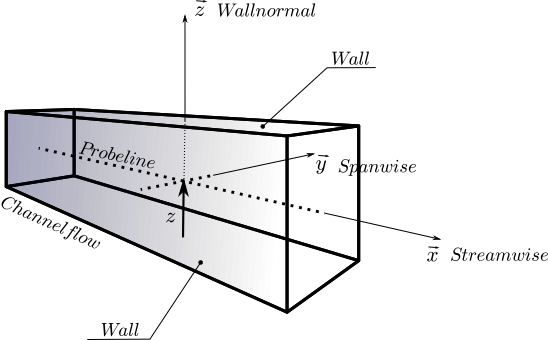
\includegraphics[width=0.62\linewidth]{../../report/referance/channel_flow.png}
		\caption{Schéma de la simulation "channel flow"}
		\label{fig:channel_flow}
	\end{center}
\end{figure}

Sur la Figure \ref{fig:channel_flow} une seul ligne de mesure dans les directions $x$ et $y$ est représentée par soucis de clarté. Dans nos simulation nous en avons utilisé entre 5 et 10 selon le modèle. Le détaille des maillages et des paramètres utilisés dans les simulations est présent dans la section suivante. \\

La Large Eddy Simulation (LES) est une méthode de simulation numérique utilisée pour résoudre les équations de Navier-Stokes en modélisant les écoulements turbulents. Contrairement aux méthodes plus simplifiées comme les Reynolds-Averaged Navier-Stokes (RANS), qui modélisent toute la turbulence, la LES se concentre sur une approche plus fine. Elle consiste à résoudre explicitement les grandes structures tourbillonnaires de l’écoulement (grandes échelles) tout en modélisant les plus petites structures (petites échelles) qui ne peuvent être capturées directement. \\
La méthode LES repose sur un filtrage spatial des équations de Navier-Stokes. Ce filtrage sépare les grandes échelles (résolues) des petites échelles (modélisées via un modèle de sous-mailles). L’idée principale est que les grandes échelles de turbulence sont spécifiques à l’écoulement et doivent être directement simulées, tandis que les petites échelles, supposées plus universelles, peuvent être modélisées avec un modèle de turbulence de sous-mailles. Au niveau des parois la résolution des petites échelles devient nécessaire et donc les méthode LES sont assez coûteuses même si le coup varie beaucoup en fonction du sous modèle choisi. \\

Dans notre étude nous avons utilisé deux sous modèles de type LES : le Wall-Resolved LES (WRLES) et le Wall-Modeled LES (WMLES). \\
Le modèle WRLES résout explicitement toutes les structures turbulentes, y compris celles présentes dans la couche limite proche des parois. Cela signifie qu’une résolution extrêmement fine est nécessaire à proximité de la paroi pour capturer les petites échelles de la turbulence. En pratique, cette approche est coûteuse, car la taille des mailles doit être très petite dans cette région, d’autant plus que le nombre de Reynolds est élevé. \\
Le modèle WMLES est une approche hybride dans laquelle on utilise un modèle de paroi (wall model) pour modéliser l’écoulement turbulent à proximité des parois, tandis que les grandes échelles turbulentes loin des parois sont résolues de manière explicite par la LES. En d'autres termes, la WMLES évite la nécessité de résoudre explicitement les petites structures turbulentes dans la couche limite, ce qui permet d'utiliser une grille plus grossière près des parois, réduisant ainsi les coûts de calcul.

\begin{center}
	\large \bf{***}
\end{center}

\vspace{0.3cm}
\section{Analyse simple des variables de vitesse turbulente afin de valider les jeux de données}
\noindent\rule{\linewidth}{2pt}
\vspace{0.1cm}

Dans cette section nous réalisons une analyse visuelle et comparative des données de sortie obtenu afin de voir si les résultats correspondent aux attentes d'une simulation d'écoulement turbulent dans un "channel flow". Les paramètres utilisées pour les trois simulations sont dans le tableau \ref{tab:parameters}: \\

\begin{table}[!h]
	\begin{tabular}{l | c | c | c}

		Grandeurs & WRLES $Re_{\tau}=395$ & WMLES $Re_{\tau}=1000$ & WRLES $Re_{\tau}=1000$\\ \hline \hline
		Dimension du canal ($x\times y \times z$) &  $2\pi\times\pi\times2$ & $4\pi\times1.5\pi\times2$ & $4\pi\times1.5\pi\times2$\\
		Masse volumique fluide &  $\rho = 1.0$ & $\rho = 1.0$ & $\rho = 1.0$ \\
		Vitesse à "l'infinie" & $u_{\infty}=1.0$ & $u_{\infty}=1.0$ & $u_{\infty}=1.0$  \\
		Grille ($N_x\times N_y \times N_z$) & $256\times128\times1936$ & $192\times96\times96$ & $640\times257\times320$ \\
		Nombre d'iteration & $N_{iter}=50000$ & $N_{iter}=75000$ & $N_{iter}=150000$ \\
		Pas de temps & $\delta t=0.01$ & $\delta t=0.01$ & $\delta t=0.004$ \\
		Nombre de Reynolds & $Re = 13800.0$ & $Re = 40000.0$ & $Re = 40000.0$ \\
		Reynolds de frottement & $Re_{tau} = 388.97$ & $Re_{tau} = 968.55$ & $Re_{tau} = 980.86$ \\
		Viscosité dynamique& $\mu = 0.000145$ & $\mu = 5e-05$ & $\mu = = 5e-05$ \\
		Viscosité cinématique & $\nu = 0.000145$ & $\nu = 5e-05$ & $\nu = 5e-05$ \\
		Vitesse de frottement & $u_{\tau} = 0.0564$ & $u_{\tau} = 0.0484275$ & $u_{\tau} = 0.0484275$ \\
		\hline
	\end{tabular}
	\caption{Paramètres des simulations numériques LES effectuées}
	\label{tab:parameters}
\end{table}


Afin de valider les résultats des calculs LES nous avions à disposition des données issues de calculs DNS (Direct Navier-Stokes) \cite{lee2015direct}. Aussi concernant le cas $Re = 395$, un calcul utilisant un modèle RANS ($k-\omega$) a été effectué. Pour que les résultats soit comparables les données ont été relevées aux même auteurs adimensionnelles que les calcules DNS (tab. \ref{tab:zplus}). \\

\begin{table}[!h]
\begin{tabular}{l | c }

	Modèles & localisation normal ($z^+$) \\	\hline	\hline
	WRLES $Re_{\tau}=395$  & $5,~20,~40,~98,~151,~199,~251,~302,~392,~$ \\
	WMLES $Re_{\tau}=1000$ & $151,~199,~251,~302,~380.04,~392,~503.63,~638.27,~762.79,~990.67$ \\
	WRLES $Re_{\tau}=1000$ & $~20,~40,~98,~151,~199,~251,~302,~380.04,~392,~503.63,~638.27,~762.79,~990.67$ \\
	\hline
\end{tabular}
	\caption{Hauteurs adimensionnelles auxquelles ont été relevées les quantités de vitesse}
	\label{tab:zplus}
\end{table}

Les grandeurs relevées auxquelles nous nous sommes intéressé dans ce travail sont les vitesses "streamwise" ($u_x, u_1 \text{ ou } u$), "spanwise" ($u_y, u_2 \text{ ou } v$) et wall-normal ($u_z, u_3 \text{ ou } w$). Nous noterons par la suite les vitesses moyennes turbulentes avec des majuscules ($U,~V,~W$) et les fluctuations turbulentes de vitesse avec des minuscules ($u,~v,~w$).\\

Regardons les profiles de vitesse moyenne et des composantes du tenseur de Reynolds ainsi que le profile d'énergie cinétique turbulente, $k_T=\frac{1}{2}(u^2+v^2+w^2)$ tracé en {\bf Figures \ref{fig:mean-vel}} et {\bf  \ref{fig:fluct-vel}}. Toutes ces vitesses ont été addimentionnées par la vitesse de frottement $u_{\tau}$. Les vitesses moyennes sont obtenues en faisant une moyenne à la fois en temps et en espace. Pour obtenir les fluctuations turbulentes on soustrait cette moyenne aux données brutes.\\

$\bullet$ Notons que dans la majorité des figures présentes dans ce rapport l'axe des ordonnées est partagé entre les sous-graphes. Il est aussi important de relever qu'afin de garder une certaine synthèse du travail et une meilleur cohérence j'ai choisit de laisser en potentiel ouverture à ce travail la comparaison des différents modèles de calcul LES. C'est pourquoi le choix à été fait de présenter uniquement les figures correspondant au modèle WRLES-$Re_{\tau}395$ même si les mêmes courbes ont pu être tracées pour les deux autres modèles à $Re=1000$ une fois que le code de calcul était terminé.

\begin{figure}[H]
	\begin{center}
		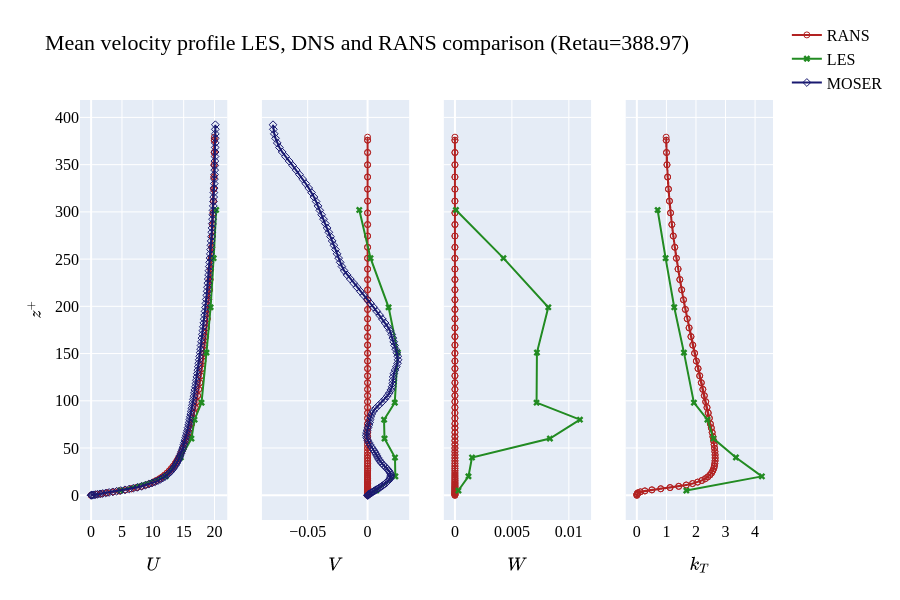
\includegraphics[width=0.8\linewidth]{../../output/figures/channel_wrles_retau395/split_time/RANS/RANS_LES_MOSER_profiles_all.png}
		\caption{Profiles de vitesse moyenne addimensionnée et d'énergie cinétique turbulente. Les données ont été comparées aux profiles des données DNS et RANS quand cela était possible.}
		\label{fig:mean-vel}
	\end{center}
\end{figure}

Nous avons un développement de la couche limite turbulente visible en regardant la vitesse moyenne $U$ de la \textbf{Figure \ref{fig:mean-vel}}. Aussi les profiles de vitesse "steamwise" sont comparables aux données DNS et RANS. Par ailleurs les vitesses "spanwise" et "wall-normal" sont petites devant cette dernière et le comparatif est donc un peu moins idéal. On observe un certain décalage dans la comparaison des composantes du tenseur de Reynolds pour celles incluant $u_2$ et $u_3$. Ces écarts sont attendu car la DNS est une méthode de résolution directe des équation de Navier-Stokes et donc les résultats sont plus précis que pour le cas de la LES où un filtrage est appliqué aux petites structures. Dans un grand nombre de cas concernant la simulation numérique appliquée à la mécanique des fluides, afin de vérifier la véracité des calculs d'un modèle ont les compare à une simulation simple calculée avec un modèle DNS considéré alors comme une solution quasi-exact. Malgré ces différences dû au modèle utilisé, les profiles de vitesse et celui d'énergie cinétique restent semblables. Nous pouvons donc considérer que ces données calculées par le modèle LES sont utilisable pour une analyse plus approfondie. \\

La même étude à été mener pour les deux modèles à Reynolds 1000. Concernant ces derniers il est intéressant de noter que l'augmentation du nombre de Reynolds à considérablement augmenté le temps de calcul entre autres pour le modèle WRLES (cf. section 4). Aussi pour chaque schéma les jeux de données était lourd (~83 Go). Il a donc fallut optimiser l'utilisation de la mémoire vive (RAM) durant le calcul. Nous avons choisit de séparer les données vis à vis des itérations en temps et au lieu d'avoir des vecteurs à 50000, 75000 et 150000 itérations en temps, ils sont de $2^10$, $2^11$ ou $2^13$ itérations (au choix de l'utilisateur et de la RAM disponible). Ensuite nous avons effectué une moyenne sur les sous groupes afin d'étudier correctement tout le jeux de données.\\

\begin{figure}[H]
	\begin{center}
		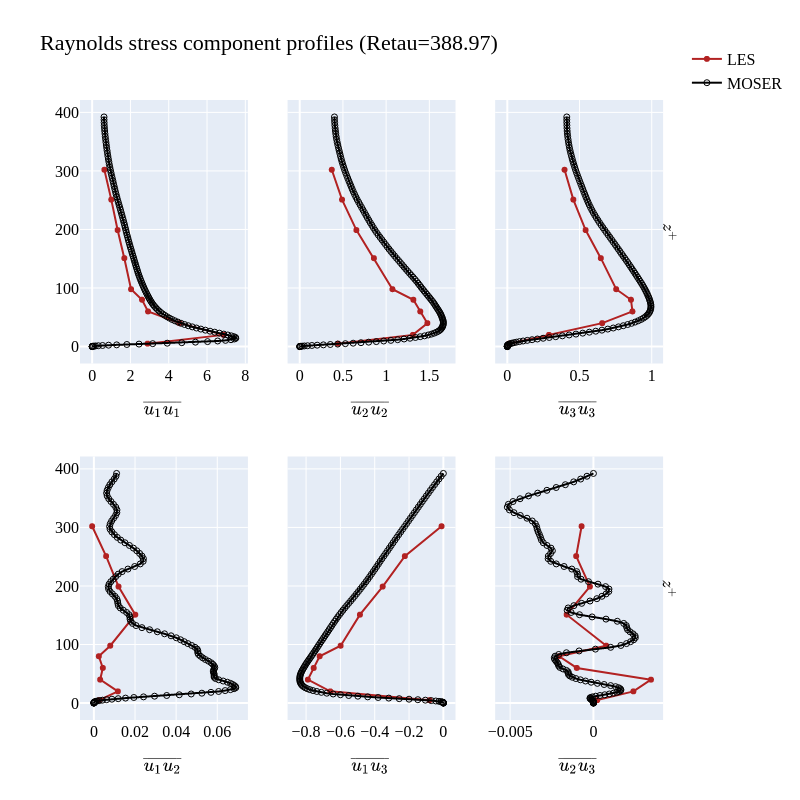
\includegraphics[width=0.8\linewidth]{../../output/figures/channel_wrles_retau395/split_time/RANS/var_velocity_profiles_all.png}
		\caption{Profiles de fluctuation. Les données ont été comparées au profiles des données DNS.}
		\label{fig:fluct-vel}
	\end{center}
\end{figure}

Les jeux de données semblant correctes nous allons pouvoir nous intéresser à l'hypothèse de turbulence figée (prop. \ref{prop:turb-fig}). Dans la théorie de résolution numérique des équation de la turbulence cette hypothèse est fait. Nous voulons donc voir si les résultats du calcul la confirme. 



\begin{center}
	\large {\bf{***}}
\end{center}

\vspace{0.3cm}
\section{Validation de l'hypothèse de turbulence figée}
\noindent\rule{\linewidth}{2pt}
\vspace{0.1cm}

Pour cette section nous nous appuierons sur l'équation \ref{fig:turb-fig} qui traduit mathématiquement l'hypothèse de turbulence figée. Nous voulons vérifier que le spectre calculé par rapport à l'espace est, à une constante près, égale au spectre calculé par rapport au temps. Cette constante correspond à la vitesse de convection moyenne du fluide dans le sens de son écoulement dans le canal qu'on notera $U_c$. Il faut donc tout d'abord trouver cette constante. Pour cela nous allons calculer la fonction d'autocorrelation bidimensionnelle $R(\delta t, \delta x)$ et tracer ses iso-valeurs sur le plan ($\delta x, \delta t$) ({\bf Figure \ref{fig:corr-2d}}). La pente définie par la direction des ellipses correspond à $\frac{1}{U_c}$.

\begin{figure}[H]
	\begin{center}
		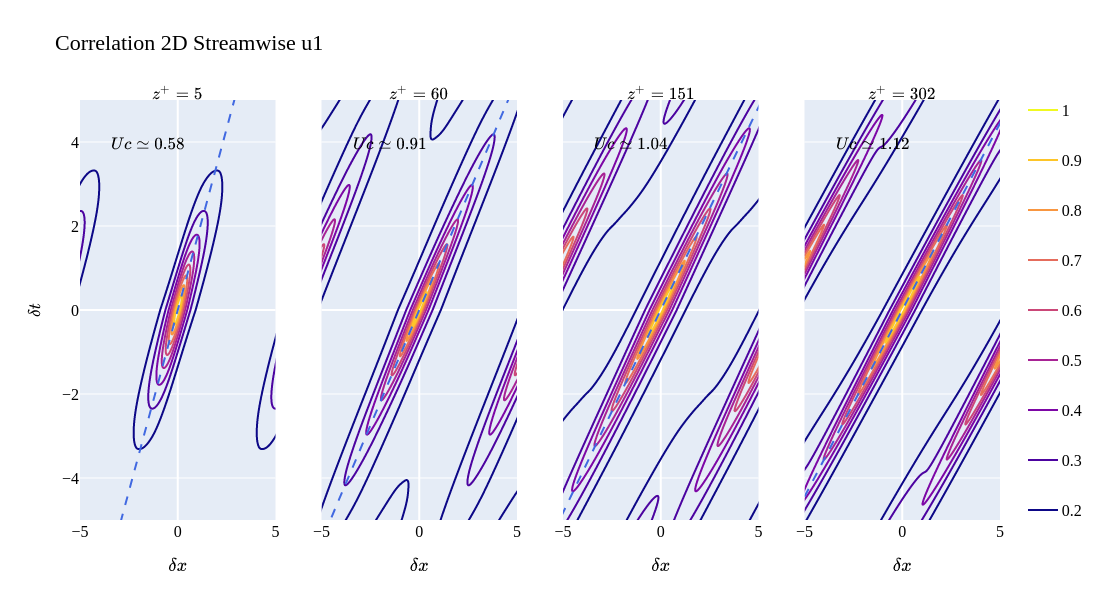
\includegraphics[width=0.9\linewidth]{../../output/figures/channel_wrles_retau395/split_time/frozen_turbulence/correlation2D/u1.png}
		\caption{Iso-valeur de la fonction d'autocorrelation 2D selon la direction $x$ et le temps $t$ à différentes hauteurs $z^+$. Obtention de la valeur de $U_c$ par approche linéaire de la direction des ellipses.}
		\label{fig:corr-2d}
	\end{center}
\end{figure}

Les valeurs de $U_c$ trouvées doivent se rapprocher des valeurs moyennes de vitesse "streamwise" $U_1$ (cf. {\bf Annexe Figure \ref{fig:comp_u1_uc}}).\\

À présent on calcule le spectre selon le nombre d'onde $k$ (espace) et
selon la fréquence $\omega$ (temps) en utilisant la méthode de Welch \cite{welch1967spectra} avec une fenêtre de "hann". En regardant la {\bf Figure \ref{fig:spectra-space-time}} les deux spectres se superposent. On pourra remarquer que la courbe en temps (en bleue) est d'avantage bruité que celle en espace (en rouge). Cela est du au nombre d'itération plus nombreuses en temps qu'en espace.
Au regard de cette figure il est possible de conclure que l'équation \ref{fig:turb-fig} est vérifiée et que l'hypothèse de turbulence figée est donc bien admissible dans notre simulation.

\begin{figure}[H]
	\begin{center}
		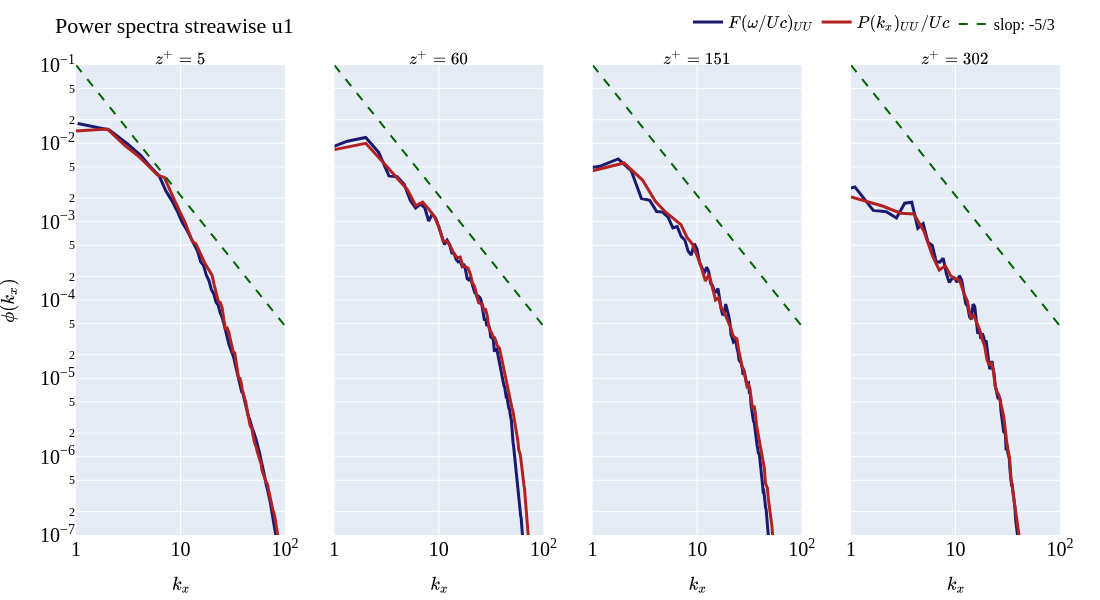
\includegraphics[width=0.85\linewidth]{../../output/figures/channel_wrles_retau395/split_time/frozen_turbulence/power_spectra/u1.png}
		\caption{Comparaison des spectres de puissance en temps ($F$) et dans la direction $x$ ($P$) tracer en fonction de $k_x$ le nombre d'onde "streamwise". En pointillé (- - -) la pente $k_x^{-5/3}$ vérifiant la décroissance de Kolmogorov \cite{kolmogorov1991local}}
		\label{fig:spectra-space-time}
	\end{center}
\end{figure}


\begin{center}
	\large \bf{***}
\end{center}

\vspace{0.3cm}
\section{Détermination du coefficient de décorrélation}
\noindent\rule{\linewidth}{2pt}
\vspace{0.1cm}

Une grandeur statistique intéressante à regarder est la corrélation (Équation \ref{eq:correlation}) afin de voir son évolution en fonction de $r=\delta x$ par rapport à un point de référence.\\
Pour points de référence nous prendrons les premiers point à $x=\delta x$ à quatre hauteurs différentes. En {\bf Figure \ref{fig:space_spectra}} vous trouverez les courbes d'auto-corrélation ($R_{UU}$, $R_{VV}$, $R_{WW}$) de vitesses dans les trois directions selon les points de relevés "streamwise". En annexe est présenté la même figure mais pour les relevés "spanwise", {\bf Figure \ref{fig:space_spectra_spanwise}}. On peut remarquer que quelque soit la direction les vitesses de décorrélation sont du même ordre de grandeur. Cela montre l'homogénéité de l'écoulement dans les directions "streamwise" et "spanwise". \\


\begin{figure}[H]
	\begin{center}
		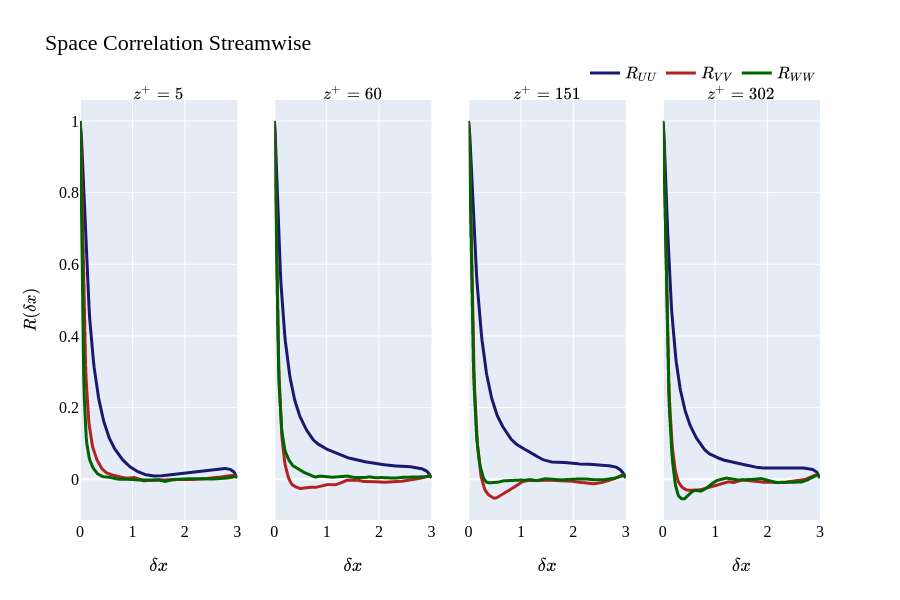
\includegraphics[width=0.8\linewidth]{../../output/figures/channel_wrles_retau395/split_time/space_correlation/streamwise.png}
		\caption{Corrélation streamwise des grandeur de vitesse dans les trois directions}
		\label{fig:space_spectra}
	\end{center}
\end{figure}

À présent nous cherchons à déterminer le coefficient de décorrélation qu'on nommera $\gamma$. Si on suppose que l'écoulement est isotrope, homogène dans la direction de détermination du coefficient et que l'hypothèse de turbulence figée est vérifiée alors il est possible de déterminer l'équation suivante: 

\begin{equation}
	\phi(r, \omega) = \frac{e^{-|\gamma k_c r| + jk_cr}}{U_c}\phi(\omega)
	\label{eq:funct}
\end{equation} 

avec $r = \delta x$, $k_c=\omega/U_c$ le nombre d'onde "streamwise", $\gamma$ le coefficient de décorrélation et $j$ le nombre imaginaire tel que $j^2=-1$. Le spectre $\phi(\omega)$ a été calculé avec la méthode de Welch et le spectre $\phi(\delta x, \omega)$ a été calculé en appliquant une transformé de Fourier à la fonction de corrélation bidimensionnelle $R_{ii}(r,\tau)$ en fonction du temps.\\
Ainsi il est possible de tracer $\beta = |\gamma k_c r|$ en fonction de $k_c$ (ou $\omega=k_c U_c$) ({\bf Figure \ref{fig:gamma_w}}) ou $r$ ({\bf Figure \ref{fig:gamma_r} Annexe}) et de déterminer $\gamma$. Dans la littérature on trouve des coefficients de décorrélation de l'ordre de $0.3$. Une fois la fonction $\beta$ tracée on a alors le coefficient de pente calculé en {\bf Figure \ref{fig:gamma_w}}, $c=\gamma r / U_c$. On peut donc déterminer le coefficient de décorrélation dont on a donné les valeurs en {\bf Figures \ref{fig:gamma_w_view}} pour les trois composantes de vitesse. \\
Il semblerait que nous n'obtenions pas le coefficient attendu, notamment pour des points très rapprochés ($r$ petits). En effet ceci ce trouve autour de $\gamma = 6$ ce qui est aberrant. Cela signifie sûrement que le modèle pris pour déterminer l'équation \ref{eq:funct} ne s'applique pas dans notre cas. Par exemple dans la réalité des mesures nous savons que l'isotropie n'est pas vérifié.



\begin{figure}[H]
	\begin{center}
		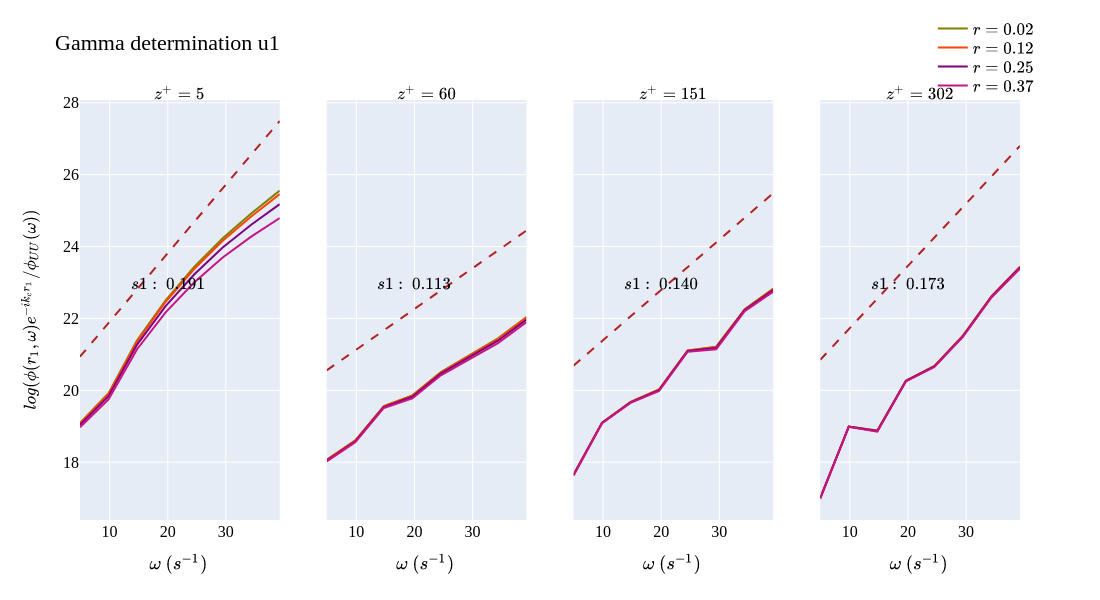
\includegraphics[width=0.9\linewidth]{../../output/figures/channel_wrles_retau395/split_time/gamma/gamma_u1_w.png}
		\caption{Tracé de la fonction $\beta$ en fonction de $k_c$ pour la vitesse $u_1$ à quatre hauteurs dans le canal et pour quatre différents $r$. Les pointillés représente la pente approchée de la courbe}
		\label{fig:gamma_w}
	\end{center}
\end{figure}



\begin{figure}[H]
	\begin{center}
		\includegraphics[width=0.8\linewidth]{../../output/figures/channel_wrles_retau395/split_time/gamma/gamma_view_w_all_mod.png}
		\caption{Évolution du coefficient de corrélation $\gamma$ en fonction de $\omega$ pour différentes distances $r$}
		\label{fig:gamma_w_view}
	\end{center}
\end{figure}


\begin{center}
	\large \bf{***}
\end{center}




\vspace{0.3cm}
\section{Comparaison des spectres avec la théorie de von Kármán}
\noindent\rule{\linewidth}{2pt}
\vspace{0.1cm}

Nous voulons maintenant comparer les résultats spectrales obtenu avec les modèles LES et les spectres obtenus avec la théorie de von Kármán explicités en section 3. Nous comparons aussi ces résultats au données DNS \cite{lee2015direct}. \\
La théorie de von Kármán s'appui sur l'hypothèse d'isotropie qui n'est pas valide dans le cas des modèles LES. Nous voulons donc quantifié les écartes en énergie que la théorie de von Kármán à avec les modèles LES et DNS. Pour cela nous utilisons les équations \ref{eq:phi_vk_1}, \ref{eq:phi_vk_2} et \ref{eq:phi_vk_3} pour calculer les spectres de densité d'énergie selon la théorie de von Kármán. Les valeurs du nombre d'onde $k_c$ et de $l$ sont obtenu à l'aide d'un calcul RANS impliquant les même paramètres. Les spectres issus des données LES sont quant à eux calculés grâce à la méthode de Welch en espace ({\bf Figure \ref{fig:vk_spectra}}). La pente de coefficient $-\frac{5}{3}$ à été tracé en pointillé sur la {\bf Figure \ref{fig:vk_spectra}} afin de vérifier la théorie de Kolmogorov. Pour une meilleur visibilité notamment pour les $z^+=60, 151, 302$ vous pouvez vous référez à la {\bf Figure \ref{fig:vk_spectra_zoom}} en annexe. \\

Les résultats LES et DNS sont quasiment similaire. Cela confirme que notre calcul LES est bon. Pour autant un écart assez conséquents ce remarque avec la théorie de von Kármán. Comme dans la théorie de von Kármán le spectre s'étand sur un nombre d'onde infinie nous remarquons que les spectres théorique sont bien plus étendus. Nous voulons donc s'avoir si la quantité d'énergie, c'est à dire mathématiquement "integral length scale", sont équivalentes. En {\bf Figure \ref{fig:vk_integral_scale}} on constate que le rapport de ces grandeurs sont entre 2 et 3. La théorie de von Kármán n'est donc pas une parfaite approximation des phénomènes de turbulence en canal pour autant dans certain cas ce modèle théorique peut rester une bonne approximation. 
	

\begin{figure}[H]
	\begin{center}
		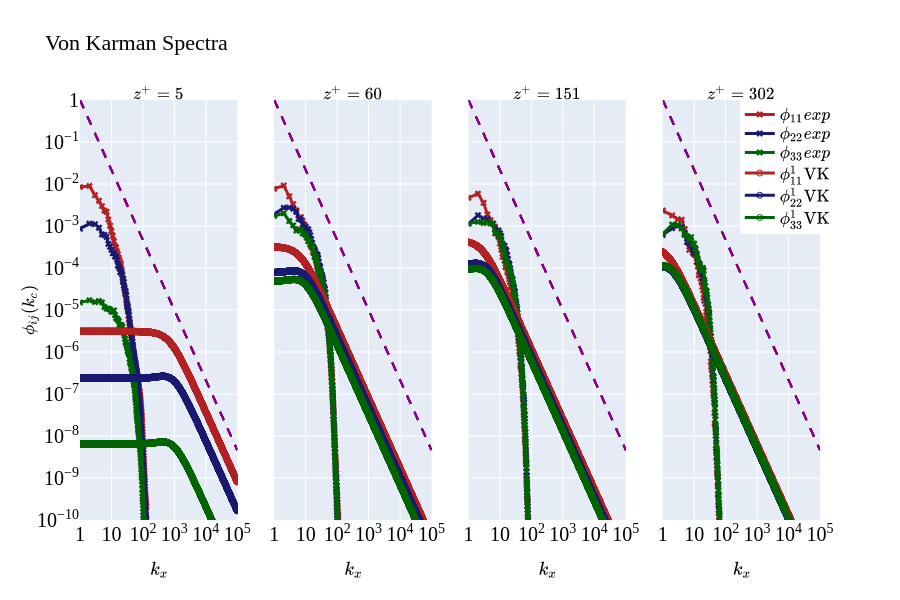
\includegraphics[width=0.9\linewidth]{../../output/figures/channel_wrles_retau395/split_time/von_karman/von_karman_spectra_.png}
		\caption{Comparaison des spectre de densité d'énergie issus de la théorie de von Kármán avec ceux issu des données LES et DNS.}
		\label{fig:vk_spectra}
	\end{center}
\end{figure}


\begin{figure}[H]
	\begin{center}
		\includegraphics[width=0.7\linewidth]{../../output/figures/channel_wrles_retau395/split_time/von_karman/integral_lenght_scale.png}
		\caption{Rapport des échelles de longueurs intégrales entre les données LES et la théorie von Kármán}
		\label{fig:vk_integral_scale}
	\end{center}
\end{figure}
	


\begin{center}
	\large \bf{***}
\end{center}

\vspace{0.3cm}
\section{Conclusion}
\noindent\rule{\linewidth}{2pt}
\vspace{0.1cm}

Notre travaille à permis dans un premier temps de valider les résultats du code LES. Par la suite nous avons vérifié une hypothèse forte, celle de turbulence figée. Avec ces deux résultats cela permet d'être confiant quant à l'utilisation des modèles WRLES et WMLES dans le cas d'une simulation en soufflerie comme celle détaillée dans le rapport. On à pu par la suit chercher à retrouver le coefficient de décorrélation. Cela n'a pas aboutit à de résultats convainquant mais pour autant il reste inintéressant vis à vis de la validité de l'équation \ref{eq:funct} dans notre cas. Pour finir nous avons pu observer les écarts entre la théorie de von Kármán et les résultats numériques LES et DES dans notre configuration. À notre connaissance, cela n'avait pas été fait auparavant et on a pu constate que dans notre cas la théorie de von Kármán ne permet pas de recouvrir toutes l'énergie que nous obtenons avec les résultats de simulation. \\ 
Dans ce rapport seulement les résultats du modèle WRLES - Retau395 on été montrés car ils ont représenté la majorité du travail effectué. Pour autant les calculs et des résultats on aussi été obtenus sur les modèles à $Re_{\tau}=1000$. De plus une comparaison entre les deux modèles WRLES et WMLES pourrait faire l'objet de suite à ce travail. En effet au niveau temps de calcul le modèle WMLES est bien plus rapide. Il faudrait donc voir si les résultats donnés par celui-ci sont assez satisfaisant par rapport au modèle WMLES afin de détermine lequel est le plus intéressant de choisir dans le cas de notre simulation. \\
L'objectif à terme est de pouvoir utiliser le code établie durant ces trois mois pour effectuer des calcules similaires sur une simulation de pâle d'éolienne en soufflerie. En revanche dans ce nouveaux cas l'écoulement n'est plus homogène dans aucune direction ce qui rend les calculs plus compliqués. Le code à été écrit de sort à ce qu'il soit modulaire et donc facilement malléable. Il serait donc assez simple, au niveau de la programmation, d'adapter le code au cas d'une pâle. En revanche il faudrait faire attention aux calculs qui n'ont plus de sens dans ce cas précis.

\pagebreak

\section{Annexe}
\noindent\rule{\linewidth}{2pt}
\vspace{0.1cm}
\subsection{Figures annexes}

Dans cette annexe j'ai seulement voulu présenter quelques figures de plus pour préciser certains points évoqué dans le rapport.

\begin{figure}[H]
	\begin{center}
		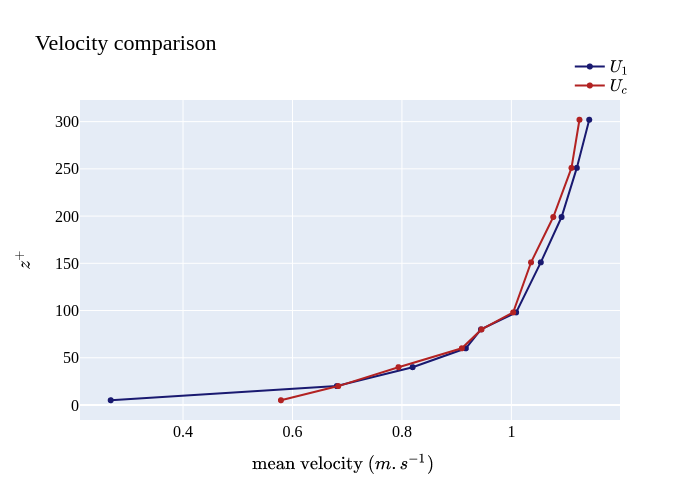
\includegraphics[width=0.8\linewidth]{../../output/figures/channel_wrles_retau395/split_time/frozen_turbulence/correlation2D/u_1c_all.png}
		\caption{Comparaison entre la vitesse d'écoulement "streamwise" obtenue par moyennage et obtenu par calcul de la pente générer par les ellipses de la corrélation 2D (Figure \ref{fig:corr-2d})}
		\label{fig:comp_u1_uc}
	\end{center}
\end{figure}

\begin{figure}[H]
	\begin{center}
		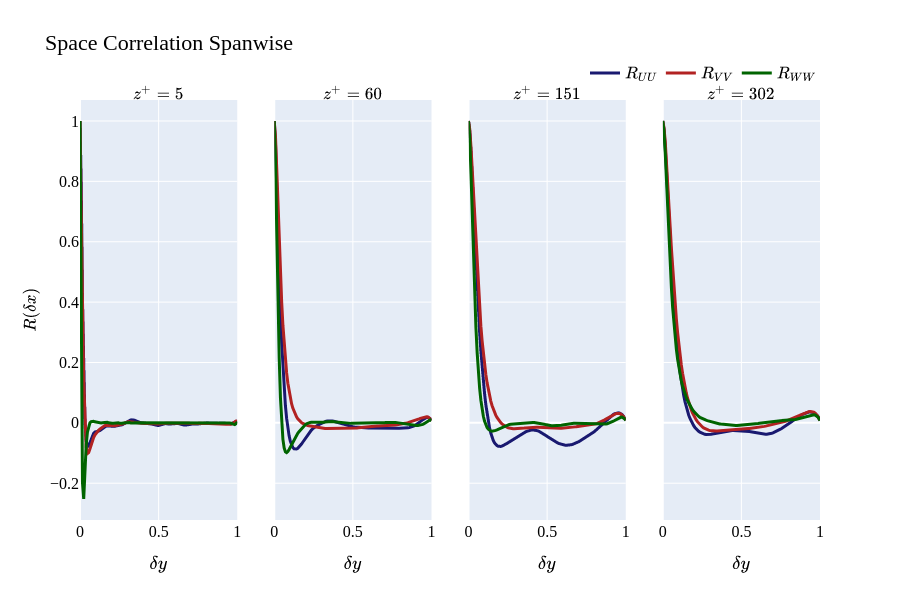
\includegraphics[width=0.9\linewidth]{../../output/figures/channel_wrles_retau395/split_time/space_correlation/spanwise.png}
		\caption{Corrélation spanwise des grandeur de vitesse dans les trois directions}
		\label{fig:space_spectra_spanwise}
	\end{center}
\end{figure}

\begin{figure}[H]
	\begin{center}
		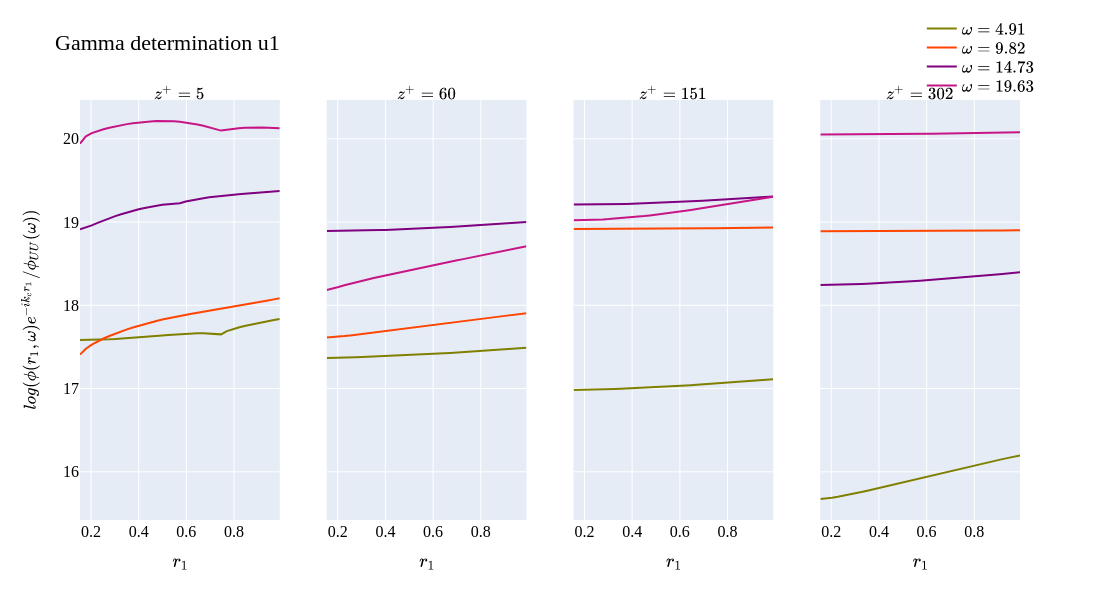
\includegraphics[width=0.9\linewidth]{../../output/figures/channel_wrles_retau395/split_time/gamma/gamma_u1_r.png}
		\caption{Tracé de la fonction $\beta$ en fonction de $r$ pour la vitesse $u_1$ à quatre hauteurs dans le canal et pour quatre différents $\omega$}
		\label{fig:gamma_r}
	\end{center}
\end{figure}

\begin{figure}[H]
	\begin{center}
		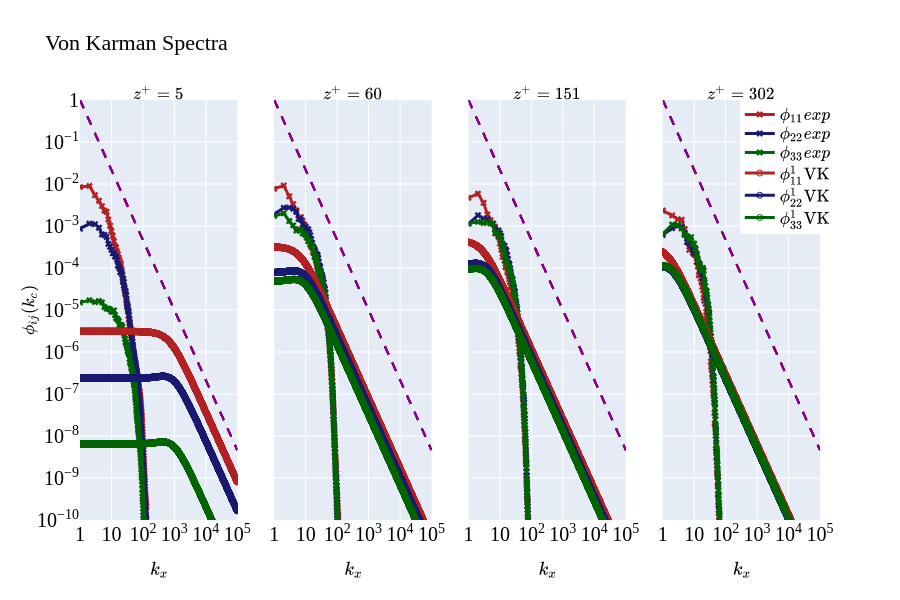
\includegraphics[width=0.9\linewidth]{../../output/figures/channel_wrles_retau395/split_time/von_karman/von_karman_spectra.png}
		\caption{Comparaison des spectre de densité d'énergie issus de la théorie de von Kármán avec ceux issu des données LES et DNS.}
		\label{fig:vk_spectra_zoom}
	\end{center}
\end{figure}

\pagebreak


\subsection{Annexe du CREGE}

Dans cette annexe nous allons détailler la gestion des projets au laboratoire DTU Wind and Energy Systems dans lequel j'ai pu effectuer mon stage. Celui-ci est un laboratoire de recherche travaillant sur plusieurs domaines de la physique et de l'ingénieurie appliqué à l'amélioration technologique des éoliennes dans le cadre d'une transition vers une énergie décarbonée. \\

Dans le laboratoire plus de 200 projets sont actuellement en cours à la fois académiques et industrielles. À DTU la part d'application industrielle des projets et mise en avant et dans de nombreux cas les chercheurs travaillent en collaboration avec des industrielles. Un accent est aussi mis sur le développement international de ces projets. Le laboratoire est représenté par des organisations danoises et internationales (ex. Wind Europe) ainsi que par des plateformes de recherche et développement travaillant dans l'énergie renouvelable. \\
De plus le campus de DTU Risø possède des équipements qui permettent aux équipes de recherche d'effectuer la majorité du travail de recherche aux même endroit en utilisant les même infrastructure. Cela permet un raccourcissement conséquent des délais et une minimisation du coût des projets. Quelque exemple d'équipement peuvent être donné comme une des plus grande soufflerie du monde, plusieurs éoliennes servant à l'expériementation ou encore un gros cluster de calcul pour la simulation numérique.\\ Tous ces atouts permettent aux projets proposés au sein du laboratoire d'être reconnus, fiancer et d'aboutir à une application industrielle concrète. \\

Cela étant dis regardons plus en détail la structure du laboratoire et intéressons nous au déroulement des projets au sein de cette entité. \\
DTU Wind and Energy Systems est structuré en 4 divisions et 20 sections toutes ayant des thèmes de travail différents en rapport avec l'éolien. Pour mieux comprendre la structure du laboratoire vous pouvez vous référer à la \textbf{Figure \ref{fig:organigrame}}

\begin{figure}[H]
	\begin{center}
		\includegraphics[width=1\linewidth]{Organogram_DTU-2024.png}
		\caption{Structuration du laboratoire DTU Wind and Energy Systems}
		\label{fig:organigrame}
	\end{center}
\end{figure}

Cette hiérarchisation permet de structurer les projets autant dans leur constitution que dans leur suivie. \\ 
Il y a deux types de projet. Les projets académiques ou de recherche qui sont proposés par une ou plusieurs personnes d'une section qui, à la suite d'une validation par le chef de section, sera présenté à la direction de la division concernée ainsi qu'au groupe d'administration de projet. On peut voir dans la \textbf{Figure \ref{fig:organigrame}} que pour la partie de managment du laboratoire, en haut de l'organigramme à droite, il y a une partie de managment de groupe et un forum de managment. Ce sont les personnes qui ont ces posts qui permettent la validation des projets et la communication avec les entreprises concernées par ceux-ci. \\
Le seconde type de projets sont industriels. Celui-ci vois le jour à la suite d'une demande d'entreprise qui propose un projet avec un cahier des charges. Ainsi le groupe de managment reçoit la demande et juge quant à la capacité du laboratoire à réaliser le projet. Il se peut que le cahier des charges soit revu avec l'entreprise si nécessaire. Si le projet est accepté alors il est proposé à une équipe du laboratoire qui travail dans le domaine le plus adapté à la demande. \\
Concernant les projets de recherche ou académiques un financement est souvent nécessaire. Il peut être assez compliqué à trouver. La demande se fait sous forme de rapport expliquant le but du projet et comment y parvenir. Alors il faut parfois faire preuve d'un peu d'ingéniosité lexicale pour rendre le projet plus attractif. \\

L'organisation des projets est fait au niveaux de la sections avec une mise en place des échéances et la répartition du travail entre les différents acteurs. Cela est souvent fait avec le chef de section, des membres des groupes de managment et du personnel de l'administration.\\

Le suivit des projets est fait à la fois au niveau de la section et au niveau de la division. Cela est majoritairement fait avec des réunions d'équipe plus ou moins espacées lors desquels l'avancement et les difficultés du projet sont présentés par l'équipe ou la personne qui travail dessus sous forme de présentation orale avec support numérique. Dans le cas où le projet est industriel alors des réunion sont organisées avec l'entreprise afin de leur présenter les avancements et de leur remettre un rapport d'état.



\pagebreak

\bibliographystyle{plain}
\bibliography{biblio.bib}	
	
\end{document}